\documentclass[a4paper,12pt]{report}

\usepackage{alltt, fancyvrb, url}
\usepackage{graphicx}
\usepackage[utf8]{inputenc}
\usepackage{float}
\usepackage{hyperref}
\usepackage{markdown}
\usepackage{menukeys} 
\usepackage{minted}
\usepackage[]{mdframed}
\usepackage{titling}
\usepackage{adjustbox}

% Questo commentalo se vuoi scrivere in inglese.
\usepackage[italian]{babel}

\usepackage[italian]{cleveref}

\begin{document}

\title{Cloudnine Manager\\
\vspace{1em}
\small Software di gestione per ristoranti in formula all-you-can-eat \\
\vspace{2em}

\includegraphics[scale=0.3]{img/icon.png}
}


\author{Luca Venturini \and Federico Bagattoni}

\date{\today}

\maketitle

\tableofcontents
\chapter{Analisi}

\section{Requisiti}
Si vuole realizzare un software per la gestione di un ristorante in formula all-you-can-eat ed alla carta.
%
Dall’interrogazione degli agenti del dominio si ricava la seguente descrizione in linguaggio naturale.
\begin{mdframed}
    L’amministratore del locale richiede di poter gestire diversi aspetti del locale: i piatti nel menù appartenenti a varie categorie (antipasti, vari tipi di sushi rolls, primi piatti caldi, crudi…), l’inventario delle materie prime presenti in cella, gli ordini e le comande create dal personale di sala ed infine la chiusura del conto ed un resoconto dei ricavi di fine turno.
Il menù deve poter essere modificato, aggiungendo o rimuovendo nuovi piatti o bevande appartenenti ad una sola categoria.
Viene tenuto conto di quali e quante materie prime sono disponibili nell’inventario del locale, al fine di sapere quali piatti possono essere cucinati, così che il personale di sala possa comunicare al cliente se un piatto non è disponibile. Inoltre si controlla quali materie prime e confezioni siano in scadenza per poterle gettare oppure quali siano quelle che scarseggiano per ordinarle dal fornitore in anticipo, evitando di esaurirle completamente.
Il personale della cucina è in grado di modificare le quantità nell’inventario togliendo quelle che ha usato durante un servizio, oltre che poter visualizzare le
Il personale del locale apre una comanda ogni volta che dei clienti si siedono ad un tavolo, ogni volta che i clienti eseguono un ordine (es. 4 pezzi del n. 75 e 5 pezzi del n. 80) questo viene aggiunto alla comanda e inviato alla cucina, poi servito. 
All’inizio del pasto i clienti scelgono tra il menù fisso all-you-can-eat ed il menù alla carta, infatti al momento della chiusura della comanda se è stata scelta la prima opzione verrà calcolato il conto sommando un menù fisso per ogni commensale oppure scegliendo la seconda opzione verranno sommati tutti i prezzi dei singoli piatti ordinati, in entrambi i casi si aggiungono i prezzi delle bevande. La scelta del menù è uguale per tutti i clienti di uno stesso tavolo, non si possono avere clienti che scelgono due menù diversi presso lo stesso tavolo. 
Al fine di facilitare il servizio il gestore ha deciso di dividere la sala in zone ognuna assegnata ad un membro del personale di sala che gestisce sempre gli stessi tavoli.
Infine le prenotazioni vengono segnate nell’agenda del ristorante ogni volta che un cliente contatta il locale. Il locale ha a disposizione un numero di coperti fisso, potendo disporli in qualsiasi combinazione di tavoli possibile.
\end{mdframed}
%AGGIUNGERE QUI QUALCOSA PER GIUSTIFICARE IL FATTO CHE NON ABBIAMO FATTO NESSUNA DISAMBIGUAZIONE
%tCAMERIERE
\section{Operazioni richieste}\label{sec:ops}
Nel DB vi sono tre classi di utenza:
\begin{itemize}
    \item Amministratori
    \item Camerieri
    \item Cuochi
\end{itemize}
\par Notiamo che gli \textit{Amministratori} hanno la possibilità di eseguire le azioni di tutti gli altri ruoli mentre i \textit{Camerieri} ed i \textit{Cuochi} sono limitati alle operazioni della loro mansione.
%
\textit{E' importante notare che le operazioni menzionate successivamente non comprendono tutte le operazioni che l'applicativo svolge.}
%
\subsection{Operazioni degli amministratori}
Un amministratore deve poter:
%
\begin{itemize}
    \item Aggiungere, rimuovere e modificare il personale
    \item Aggiungere nuove materie prime all’inventario
    \item Visualizzare le materie prime la cui quantità è sotto una certa soglia critica
    \item Visualizzare i ricavi della giornata
    \item Aggiungere, rimuovere e modificare i menu
    \item {tutte le operazioni segnate ai punti \ref{sec:waiters} e \ref{sec:cooks}}
\end{itemize}
%
Le operazioni per gli amministratori sono quindi definite nel seguente modo: 
%
\begin{itemize}
    \item \texttt{A1 "AGGIUNGI STAFF"}: aggiunge un nuovo membro del personale
    \item \texttt{A2 "RIMUOVI STAFF"}: rimuove un nuovo membro del personale 
    \item \texttt{A3 "MODIFICA STAFF"}: modifica uno o più dati riguardo ad un membro del personale
    \item \texttt{A4 "RICAVI GIORNATA"}: visualizza ricavi della giornata 
    \item \texttt{A5 "NUOVO MENU"}: aggiunge un nuovo menù 
    \item \texttt{A6 "RIMUOVI MENU"}: rimuove un menù
    \item \texttt{A7 "AGGIUNGI VIVANDA A MENU"}: aggiunge un vivanda ad un menù
    \item \texttt{A8 "RIMUOVI VIVANDA DA MENU"}: rimuove un vivanda dal menù
    \item \texttt{A9 "NUOVA VIVANDA"}: aggiunge una nuova vivanda al sistema
    \item \texttt{A10 "CANCELLA VIVANDA"}: rimuove una vivanda dal sistema
\end{itemize}
%
\subsection{Operazioni dei Camerieri}\label{sec:waiters}
%
Un cameriere deve poter:
%
\begin{itemize}
    \item Creare e modificare le comande
    \item Aggiungere, rimuovere o modificare gli ordini di una comanda
    \item Aggiungere, rimuovere o modificare le prenotazioni
    \item Visualizzare i piatti che non è possibile cucinare in un dato momento
    \item Chiudere una comanda, visualizzando il conto finale
\end{itemize}
%
Le operazioni per i camerieri sono quindi definite nel seguente modo:
%
\begin{itemize}
    \item \texttt{S1 "AGGIUNGI COMANDA"}: crea una nuova comanda generando il relativo codice ed aggiungendo il numero di coperti ed il tavolo
    \item\texttt{S2 "MODIFICA COMANDA"}: modifica uno o più parametri di una comanda 
    \item\texttt{S3 "RIMUOVI COMANDA"}: elimina una comanda dal sistema 
    \item\texttt{S4 "AGGIUNGI ORDINE"}: aggiunge un ordine ad una comanda, contenente piatti o bevande e relative quantità
    \item\texttt{S5 "RIMUOVI VIVANDA"}: elimina una vivanda da un ordine già esistente
    \item\texttt{S6 "RIMUOVI ORDINE"}: rimuove un ordine da una comanda, se la cucina non l’ha ancora iniziato a cucinare 
    \item\texttt{S7 "CHIUDI COMANDA":} chiudi una comanda, calcolando una sorta di scontrino finale 
    \item\texttt{S8 "AGGIUNGI VIVANDA"}: aggiunge una vivanda ad un ordine già esistente
\end{itemize}
%
\subsection{Operazioni dei Cuochi}\label{sec:cooks}
Un cuoco deve poter:
%
\begin{itemize}
    \item Rimuovere quantità di materie prime dall'inventario quando se ne fa utilizzo
    \item Visualizzare le materie prime scadute
    \item Aggiungere una materia prima nuova o già esistente all'inventare
    \item Visualizzare le materie prime insufficienti
\end{itemize}
Le operazioni per i cuochi sono quindi definite nel seguente modo:
%
\begin{itemize}
    \item\texttt{K1 "RIMUOVI MATERIA PRIMA":} Rimuovere una certa quantita di materia prima
    \item\texttt{K2 "MATERIE PRIMA SCADUTE":} Visualizzare le materie prime scadute
    \item\texttt{K3 "AGGIUNGI MATERIA PRIMA":} aggiungere una certa quantita di materia prima
    \item\texttt{K4 "MATERIE PRIMA INSUFFICIENTI":} Visualizzare le materie prime insufficienti
\end{itemize}
%
\subsection{Operazioni di tutti gli agenti}\label{sec:everyone_ops}
Le operazioni che tutti gli agenti del dominio possono svolgere sono: 
\begin{itemize}
    \item Prendere prenotazioni
\end{itemize}
Che si traducono in:
\begin{itemize}
    \item \texttt{S9 "AGGIUNGI PRENOTAZIONE"}: aggiunge una nuova prenotazione
\end{itemize}
%
\chapter{Progettazione concettuale}
\section{Schema iniziale}
Di seguito viene riportato uno schema scheletro che verrà espanso nelle sezioni successive. Questo include le entità fondamentali dello schema:
\begin{itemize}
    \item una vivanda
    \item un ordine
    \item una comanda 
    \item un membro del personale
\end{itemize}
%
\begin{figure}[H]
    \centering
    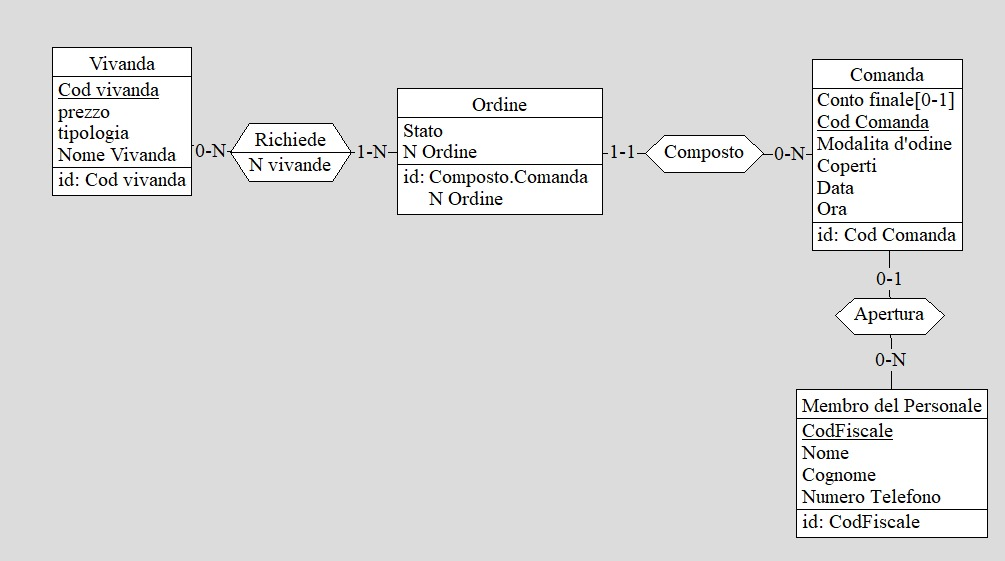
\includegraphics[width=0.95\linewidth]{img/er/iniziale.jpg}
    \caption{lo schema E-R iniziale.}
    \label{fig:iniziale-er}
\end{figure}
%
\section{Raffinamenti proposti}
%
\subsection{Membri del personale}
Al fine di specificare i ruoli all’interno del ristorante si propone la seguente gerarchia:
%
\begin{figure}[H]
    \centering
    \includegraphics[width=0.5\linewidth]{img/er/personale.jpg}
    \caption{differenziazione dei membri del personale.}
\end{figure}
%
\subsection{Menù e categorie delle vivande}
%
Visto che la peculiarità del ristorante è la diversità in termini di piatti e categorie il sistema deve permettere l’esistenza di diversi menù ognuno proposto in giornate e servizi diversi.
%
\begin{figure}[H]
    \centering
    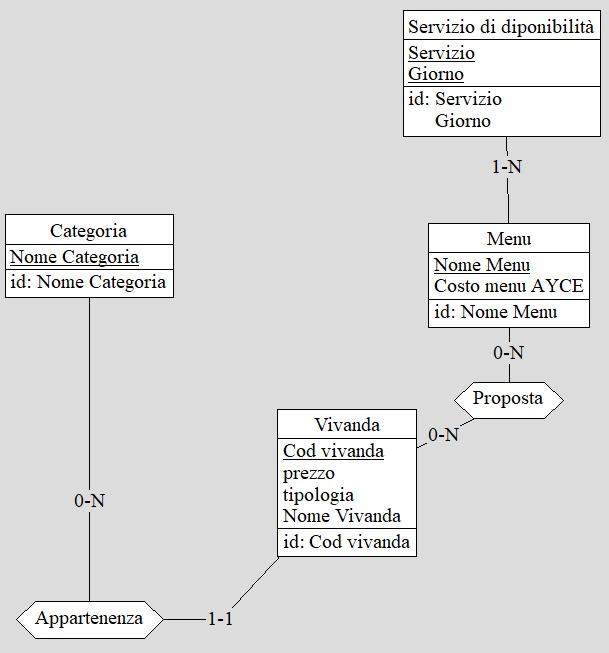
\includegraphics[width=0.8\linewidth]{img/er/vivande.jpg}
    \caption{modellazione del menù e delle categorie di piatti al suo interno.}
\end{figure}
%
\subsection{Inventario e ricette}
%
Un requisito del sistema deve essere quello di tenere conto della quantità di materie prime disponibili in cucina, questo è reso possibile modellando le materie prime necessarie a cucinare un piatto.
%
\begin{figure}[H]
    \centering
    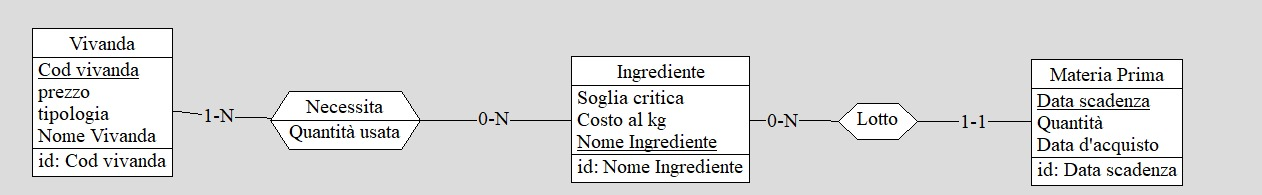
\includegraphics[width=\linewidth]{img/er/inventario.jpg}
    \caption{modellazione dell'inventario e della gestione delle materie prime.}
\end{figure}
%
\subsection{Gestione delle prenotazioni}
%
La gestione delle prenotazioni per una determinata data ed un certo turno è così modellata. 
%
\begin{figure}[H]
    \centering
    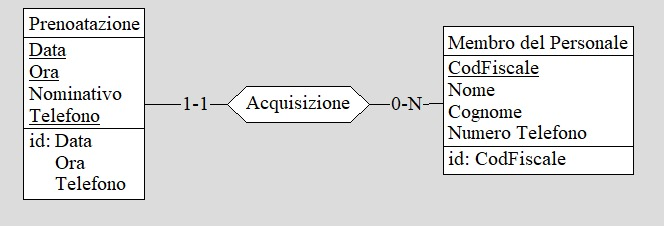
\includegraphics[width=0.7\linewidth]{img/er/prenotazioni.jpg}
    \caption{gestione delle prenotazioni.}
\end{figure}
%
\section{Schema finale}
%
Lo schema dopo l'applicazione dei raffinamenti è il seguente.
%
\begin{figure}[H]
    \centering
    \rotatebox[origin=c]{90}{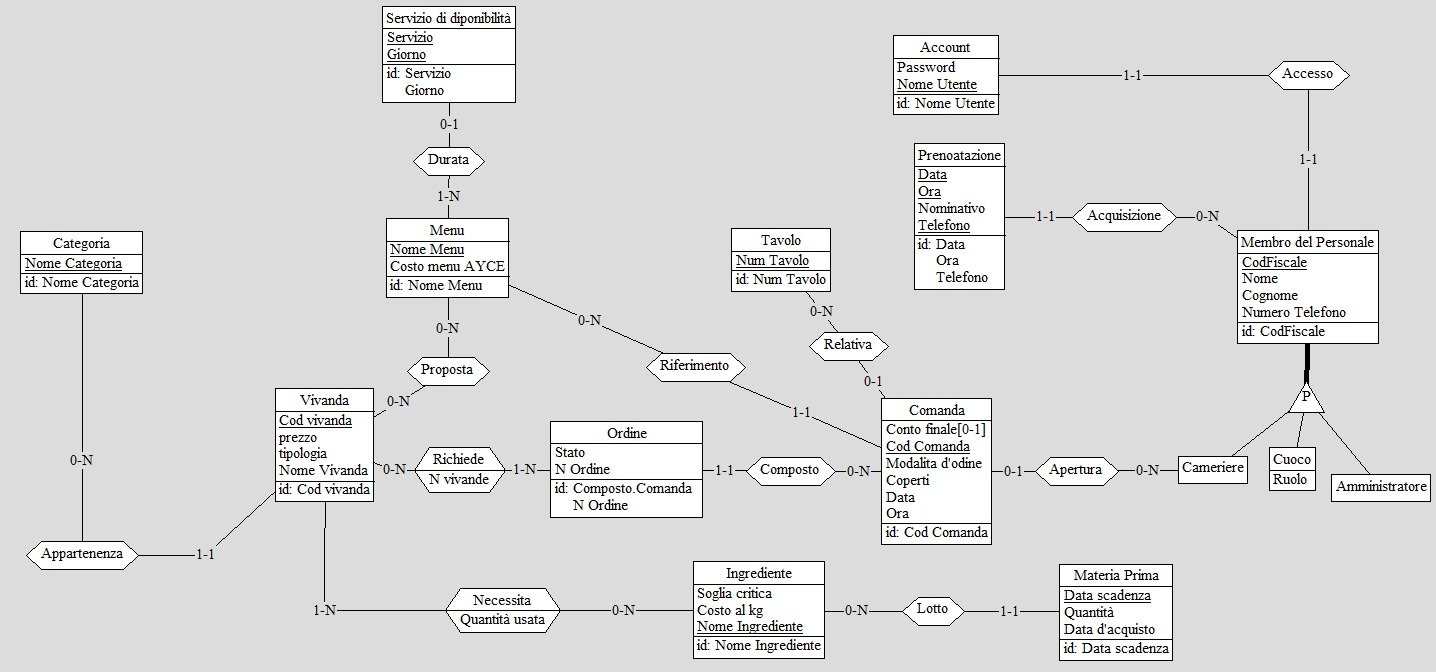
\includegraphics[width=1.5\linewidth]{img/er/finale.jpg}}
    \caption{Schema relazionale dopo l'appplicazione dei raffinamenti.}
\end{figure}
%
\section{Vincoli inespressi}
%
Bisogna osservare che lo schema ha dei vincoli inespressi che devono essere verificati tramite query:
\begin{itemize}
    \item non possono esistere più menu con lo/gli stesso/i giorni di disponibilità
    \item la data e l'ora di una comanda devono essere coerenti con il giorni di disponibilità del menu da cui sono stati ordinati i piatti contenuti negli ordini relativi alla suddetta comanda
    \item data ed ora di una prenotazione devono essere relativi a data e servizio del tavolo con cui quella prenotazione è legata
\end{itemize}
%
\chapter{Progettazione logica}
\section{Stima del volume dei dati}
In tabella \ref{table:stima-dati} viene riportata la stima del volume dei dati per ogni entità e relazione presente nello schema. Si stima l'utilizzo del sistema da parte di una modesta impresa di 8 persone e 50 coperti.
\begin{table}[H]
\centering
\begin{tabular}{||c | c | c||} 
 \hline
 Concetto & Tipologia & Volume\\
 \hline\hline
Membro del personale & E & 8\\
\hline
Cameriere &  E& 4\\
\hline
Cuoco & E& 3\\
\hline
Amministratore & E& 1\\
\hline
Account & E& 8\\
\hline
Accesso & R& 8\\
\hline
Prenotazioni & E & 35\\
\hline
Acquisizioni & R & 5\\
\hline
Tavolo & E & 12\\
\hline
Agenda & R & 35\\
\hline
Comanda & E& 2700\\
\hline
Riferimento & E & 2700\\
\hline
Apertura & R& 2600\\
\hline
Ordine & E& 5400\\
\hline
Composto & R& 2700\\
\hline
Richiede & E& 32400\\
\hline
Vivande & R& 100\\
\hline
Bevanda & E& 20\\
\hline
Consumo & R & 20\\
\hline
Piatto & R & 80\\
\hline
Necessita & R & 320\\
\hline
Ingrediente & E & 60\\
\hline
Lotto & R & 150\\
\hline
Materia prima & E & 150\\
\hline
Categorie & E & 9\\
\hline
Appartenenza & R & 100\\
\hline
Menu & E & 3\\
\hline
Proposta & R & 240\\
\hline
Divisione & R & 27\\
\hline
Periodo di disponibilità & E & 3\\
\hline
\end{tabular}
\caption{stime del volume dei dati}
\label{table:stima-dati}
\end{table}
\section{Descrizione delle operazioni principali e stima della loro frequenza}
In tabella \ref{table:stima-frequenze} sono riportate le frequenze delle operazioni previste dal sistema. Fare riferimento alla sezione \ref{sec:ops} per una descrizione più accurata delle operazioni.

\begin{table}[H]
\begin{center}
\begin{tabular}{||c | c | c | c ||} 
 \hline
 Operazione & Descrizione & Tipologia & Frequenza\\
 \hline\hline
    \texttt{A1} & Aggiunge un nuovo membro del personale & I & 2 all'anno \\
    \texttt{A2} & Rimuove un membro del personale & I & 2 all'anno\\
    \texttt{A3} & Modifica i dati di un utente & I & 3 all'anno\\
    \texttt{A4} & Visualizza ricavi della giornata & I & 1 al giorno\\
    \texttt{A5} & Aggiunge un nuovo menù & I & 4 all'anno\\
    \texttt{A6} & Rimuove un menù & I & 4 all'anno \\
    \texttt{A7} & Aggiunge una vivanda ad un menù & I & 10 all'anno\\
    \texttt{A8} & Rimuove una vivanda dal menù & I & 10 all'anno\\
    \texttt{A9} & Aggiunge una nuova vivanda al sistema & I & 10 all'anno\\
    \texttt{A10} & Rimuove una vivanda dal sistema & I & 10 all'anno\\
    \texttt{S1} & Crea una nuova comanda  & I & 40 al giorno\\
    \texttt{S2} & Modifica una comanda & I & 20 al giorno \\
    \texttt{S3} & Elimina una comanda dal sistema & I & 5 al giorno\\
    \texttt{S4} & Aggiunge un ordine ad una comanda & I & 100 al giorno\\
    \texttt{S5} & Rimuovi una vivanda da un ordine & I & 10 al giorno\\
    \texttt{S6} & Rimuove un ordine da una comanda & I & 10 al giorno\\
    \texttt{S7} & Chiudi una comanda & I & 90 al giorno\\
    \texttt{S8} & Aggiungi una vivanda ad un ordine & I & 10 al giorno\\
    \texttt{S9} & Aggiungi prenotazione & I & 10 al giorno\\
    \texttt{K1} & Rimuove una certa quantità di una materia prima & I & 200 al giorno\\
    \texttt{K2} & Visualizza le materie prime non più utilizzabili & I & 1 al giorno\\
    \texttt{K3} & Aggiunge una materia prima all’inventario & I & 30 volte al giorno\\
    \texttt{K4} & Visualizza materie prima critica & I & 1 al giorno\\
    \hline
\end{tabular}
\end{center}
\caption{stima della frequenza delle operazioni}
\label{table:stima-frequenze}
\end{table}

\section{Schemi di navigazione e tabelle degli accessi}
Certe operazioni non vengono prese in esame in quanto operano su poche entità/relazioni ed hanno costo minimo. Altre operazioni vengono direttamente calcolate e valutate nella sezione \ref{sec:redun} sulle ridondanze.
\subsubsection{A1: aggiunge un membro del personale}
\begin{table}[H]
    \centering
    \begin{tabular}{|| c | c | c | c ||}
        \hline
        Concetto & Costrutto & Accesso & Tipo\\
        \hline
        Membro del personale & E & 1 & S\\
        \hline
        Accesso & R & 1 & S\\
        \hline
        Account & E & 1 & S\\
        \hline
    \end{tabular}
\end{table}
%
Per un costo di:
%
\begin{equation}
    3\text{ S}=  9 \cdot 2 = 18\text{/anno}
\end{equation}
E' contestualmente simile l'operazione \texttt{A2}.
\subsubsection{S3: elimina una comanda}
\begin{table}[H]
    \centering
    \begin{tabular}{|| c | c | c | c ||}
        \hline
        Concetto & Costrutto & Accesso & Tipo\\
        \hline
        Comanda & E & 1 & S\\
        \hline
        Comanda & E & 1 & L\\
        \hline
        Relativa & R & 1 & L\\
        \hline
        Relativa & R & 1 & S\\
        \hline
        Tavolo & R & 1 & L\\
        \hline
        Tavolo & R & 1 & S\\
        \hline
        Composto & E & 2 & L\\
        \hline
        Composto & E & 2 & S\\
        \hline
        Ordine & E & 2 & L\\
        \hline
        Ordine & E & 2 & S\\
        \hline
        Richiede & E & \begin{math}2 \cdot 12\end{math} & L \\
        \hline
        Richiede & E & \begin{math}2 \cdot 12\end{math} & S\\
        \hline
        Riferimento & E & 1 & S\\
        \hline
        Riferimento & E & 1 & L\\
        \hline
    \end{tabular}
\end{table}
%
Per un costo di:
%
\begin{equation}
    (8 + 2 \cdot 12 ) \text{S} + (8 + 2 \cdot 12 ) \text{L}
 =  96 \cdot 5 = 480\text{/giorno}
\end{equation}
\subsubsection{S4: aggiungi un ordine ad una comanda}
%
\begin{table}[H]
    \centering
    \begin{tabular}{|| c | c | c | c ||}
        \hline
        Concetto & Costrutto & Accesso & Tipo\\
        \hline
        Comanda & E & 1 & L\\
        \hline
        Composto & A & 1 & S\\
        \hline
        Ordine & E & 1 & S\\
        \hline
        Vivanda & E & 12 & L\\
        \hline
        Richiede & A & 12 & S\\
        \hline
    \end{tabular}
\end{table}
%
Per un costo di:
%
\begin{equation}
    ((1+12)\text{L} + (1+1+12)\text{S}) = 41 \cdot 100 = 4100\text{/giorno}
\end{equation}
%
\subsubsection{S5: rimuovi vivanda dall'ordine}
\begin{table}[H]
    \centering
    \begin{tabular}{|| c | c | c | c ||}
        \hline
        Concetto & Costrutto & Accesso & Tipo\\
        \hline
        Ordine & E & 1 & L\\
        \hline
        Richiede & R & 1 & L\\
        \hline
        Richiede & R & 1 & S\\
        \hline
        Vivanda & E & 1 & L\\
        \hline
    \end{tabular}
\end{table}
%
\begin{equation}
    ((1+1)\text{L} + (1)\text{S}) = 4 \cdot 10 = 40\text{/giorno}
\end{equation}
%
\subsubsection{S6: rimuove un ordine da una comanda}
%
\begin{table}[H]
    \centering
    \begin{tabular}{|| c | c | c | c ||}
        \hline
        Concetto & Costrutto & Accesso & Tipo\\
        \hline
        Comanda & E & 1 & L\\
        \hline
        Composto & R & 1 & L\\
        \hline
        Composto & R & 1 & S\\
        \hline
        Ordine & E & 1 & L\\
        \hline
        Ordine & E & 1 & S\\
        \hline
        Richiede & R & 12 & L\\
        \hline
        Richiede & R & 12 & S\\
        \hline
    \end{tabular}
\end{table}
%
\begin{equation}
    ((1+1+1+12)\text{L} + (1+1+12)\text{S}) = 43 \cdot 10 = 430\text{/giorno}
\end{equation}
%
\subsubsection{S7: visualizza i piatti che non è possibile cucinare}
\begin{table}[H]
    \centering
    \begin{tabular}{|| c | c | c | c ||}
        \hline
        Concetto & Costrutto & Accesso & Tipo\\
        \hline
        Piatto & E & 80 & L\\
        \hline
        Necessita & R & 320 & L\\
        \hline
        Ingrediente & E & 60 & L\\
        \hline
    \end{tabular}
\end{table}
%
Per un costo di:
%
\begin{equation}
    (100 + 320 + 60) \text{L} = 480 \cdot 10 = 4800\text{/giorno}
\end{equation}
%
\subsubsection{S7-bis: visualizza le bevande non disponibili}
\begin{table}[H]
    \centering
    \begin{tabular}{|| c | c | c | c ||}
        \hline
        Concetto & Costrutto & Accesso & Tipo\\
        \hline
        Bevande & E & 20 & L\\
        \hline
        Consumo & R & 20 & L\\
        \hline
        Mageria prima & R & 20 & L\\
        \hline
    \end{tabular}
\end{table}
%
Per un costo di:
%
\begin{equation}
    60 \text{L} = 60 \cdot 10 = 600\text{/giorno}
\end{equation}
%
\subsubsection{S9: aggiungi una vivanda ad un ordine}
\begin{table}[H]
    \centering
    \begin{tabular}{|| c | c | c | c ||}
        \hline
        Concetto & Costrutto & Accesso & Tipo\\
        \hline
        Ordine & E & 1 & L\\
        \hline
        Richiede & R & 1 & S\\
        \hline
        Vivanda & R & 1 & L\\
        \hline
    \end{tabular}
\end{table}
%
Per un costo di:
%
\begin{equation}
    2\text{L} + 1\text{S} = 4 \cdot 10 = 40\text{/giorno}
\end{equation}
%
\subsubsection{S10: aggiungi una prenotazione}
%
\begin{table}[H]
    \centering
    \begin{tabular}{|| c | c | c | c ||}
        \hline
        Concetto & Costrutto & Accesso & Tipo\\
        \hline
        Prenotazione & E & 1 & S\\
        \hline
        Prenotazione & R & 1 & S\\
        \hline
        Membro del personale & E & 1 & L\\
        \hline
        Acquisizione & R & 1 & S\\
        \hline
    \end{tabular}
\end{table}
%
Per un costo di: 
%
\begin{equation}
    1\text{L} + 3\text{S} = 7 \cdot 10 = 7\text{/giorno}
\end{equation}
%
\section{Raffinamento dello schema}
Si propongono i seguenti raffinamenti:
\begin{itemize}
    \item Collasso verso l'alto della gerarchia sul personale con la creazione del vincolo inespresso per cui solo un cameriere può aprire una comanda
    \item Collasso verso l'alto della gerarchia riguardo alle vivande con l'introduzione dell'attributo \texttt{tipo}. D'ora in poi una bevanda può fare utilizzo di più ingredienti.
\end{itemize}
\section{Analisi delle ridondanze}\label{sec:redun}
Le ridondanze presenti in questo schema sono: l'attributo \texttt{quantità} nella entità \texttt{Ingrediente} il quale potrebbe essere calcolato contando \texttt{Materia prima} e l'attributo \texttt{conto finale} di \texttt{Comanda} che potrebbe essere ricavato dagli ordini eseguiti per una certa comanda quando si va a cercare il ricavo a fine serata. 
\subsection{Analisi della ridondanza di \texttt{conto finale}}
%
Le operazioni interessate sono \texttt{S8} e \texttt{A4}.
%
\paragraph{Caso con ridondanza}: per quanto riguarda il calcolo dei ricavi sarà sufficiente leggere l'attributo \texttt{conto finale} da tutte le comande mentre nell'operazione del calcolo del totale di una comanda si deve
%
\subsubsection{A4}
Questa operazione viene svolta a fine servizio per determinare i ricavi della giornata.
%
\begin{table}[H]
    \centering
    \begin{tabular}{|| c | c | c | c ||}
        \hline
        Concetto & Costrutto & Accesso & Tipo\\
        \hline
        Comanda & E & 90 & L\\
        \hline
    \end{tabular}
\end{table}
%
Per un costo di:
\begin{equation}
    90\text{/giorno}
\end{equation}
%
\subsubsection{S8}
% 
In caso di un menu all you can eat:
\begin{table}[H]
    \centering
    \begin{tabular}{|| c | c | c | c ||}
        \hline
        Concetto & Costrutto & Accesso & Tipo\\
        \hline
        Comanda & E & 1 & L\\
        \hline
        Comanda & E & 1 & S\\
        \hline
        Riferimento & R & 1 & L\\
        \hline
        Menù & E & 1 & L\\
        \hline
        Composto & R & 2 & L\\
        \hline
        Ordine & E & 2 & L\\
        \hline
        Richiede & R & 4 & L\\
        \hline
        Vivanda & E & 4 & L\\
        \hline
    \end{tabular}
\end{table}
\begin{equation}
    (1+1+1+2+2+4+4)\text{L} + 1\text{S} = 17 \cdot 80 = 1360\text{/giorno}
\end{equation}
%
In caso di un menu alla carta:
\begin{table}[H]
    \centering
    \begin{tabular}{|| c | c | c | c ||}
        \hline
        Concetto & Costrutto & Accesso & Tipo\\
        \hline
        Comanda & E & 1 & L\\
        \hline
        Comanda & E & 1 & S\\
        \hline
        Composto & R & 2 & L\\
        \hline
        Ordine & E & 2 & L\\
        \hline
        Richiede & R & 24 & L\\
        \hline
        Vivanda & E & 24 & L\\
        \hline
    \end{tabular}
\end{table}
\begin{equation}
    (1+2+2+24+24)\text{L} + 1\text{S}= 55 \cdot 10 = 550\text{/giorno}
\end{equation}
%
\paragraph{Caso senza ridondanza}: calcolando i ricavi ora bisogna calcolare gli importi delle comande.
\subsubsection{A4}
%
Ora è necessario calcolare tutte le comande, similmente al punto successivo, infatti se non si mantiene l'attributo allora si dovrà calcolare nuovamente tutte le comande: 
\begin{equation}
    1200 + 530 = 1730\text{/giorno}
\end{equation}
%
\subsubsection{S8}
%
Per un menu all you can eat:
\begin{table}[H]
    \centering
    \begin{tabular}{|| c | c | c | c ||}
        \hline
        Concetto & Costrutto & Accesso & Tipo\\
        \hline
        Comanda & E & 1 & L\\
        \hline
        Riferimento & R & 1 & L\\
        \hline
        Menù & E & 1 & L\\
        \hline
        Composto & R & 2 & L\\
        \hline
        Ordine & E & 2 & L\\
        \hline
        Richiede & R & 4 & L\\
        \hline
        Vivanda & E & 4 & L\\
        \hline
    \end{tabular}
\end{table}
%
Per un costo di:
\begin{equation}
    (1+1+1+2+2+4+4)\text{L}= 15\cdot 80 = 1200\text{/giorno}
\end{equation}
%
Per un menu alla carta:
\begin{table}[H]
    \centering
    \begin{tabular}{|| c | c | c | c ||}
        \hline
        Concetto & Costrutto & Accesso & Tipo\\
        \hline
        Comanda & E & 1 & L\\
        \hline
        Composto & R & 2 & L\\
        \hline
        Ordine & E & 2 & L\\
        \hline
        Richiede & R & 24 & L\\
        \hline
        Vivanda & E & 24 & L\\
        \hline
    \end{tabular}
\end{table}
%
Per un costo di:
\begin{equation}
    (1+2+2+24+24)\text{L} = 53 \cdot 10 = 530\text{/giorno}
\end{equation}
%
Quindi questa operazione costa:
\begin{equation}
    1200 + 530 = 1730 \text{/giorno}
\end{equation}
\subsubsection{Conclusione}
Il caso senza ridondanza costa:
\begin{equation}\label{eq:senza_rid_conto}
    1730 + 1730 = 3460 \text{/giorno}
\end{equation}
Mentre nel caso con ridondanza queste due operazioni costano: 
\begin{equation}\label{eq:con_rid_conto}
    90 + 1360 + 550 = 2020 \text{/giorno}
\end{equation}
Dati i numeri delle equazioni \ref{eq:senza_rid_conto} e \ref{eq:con_rid_conto} si conclude che il caso con ridondanza è quello più conveniente.
\subsection{Analisi della ridondanza di \texttt{quantità totale}}
Le operazioni interessate sono \texttt{K1}, \texttt{K3}, \texttt{K4}.
%
\subsubsection{Caso con ridondanza}
%
\subsubsection{K1: rimuove una certa quantità di una materia prima}
%
\begin{table}[H]
    \centering
    \begin{tabular}{|| c | c | c | c ||}
        \hline
        Concetto & Costrutto & Accesso & Tipo\\
        \hline
        Materia prima & E & 1 & L\\
        \hline
        Materia prima & E & 1 & S\\
        \hline
        Ingrdiente & E & 1 & L\\
        \hline
        Ingrediente & E & 1 & S\\
        \hline
        Lotto & R & 1 & L\\
        \hline
    \end{tabular}
\end{table}
%
\begin{equation}
    (1+1)\text{S} + (1+1+1)\text{L}= 7 \cdot 200 = 1400\text{/giorno}
\end{equation}
%
\subsubsection{K3: aggiunge una certa quantità di una materia prima}
%
\begin{table}[H]
    \centering
    \begin{tabular}{|| c | c | c | c ||}
        \hline
        Concetto & Costrutto & Accesso & Tipo\\
        \hline
        Materia prima & E & 1 & S\\
        \hline
        Ingrdiente & E & 1 & L\\
        \hline
        Ingrediente & E & 1 & S\\
        \hline
        Lotto & R & 1 & S\\
        \hline
    \end{tabular}
\end{table}
%
\begin{equation}
    1\text{L} + (1+1+1)\text{S}= 7 \cdot 30 = 210\text{/giorno}
\end{equation}
%
\subsubsection{K4: visualizza materia prima critica}
\begin{table}[H]
    \centering
    \begin{tabular}{|| c | c | c | c ||}
        \hline
        Concetto & Costrutto & Accesso & Tipo\\
        \hline
        Ingrediente & E & 60 & L\\
        \hline
    \end{tabular}
\end{table}
Per un costo di: 
\begin{equation}
    60\text{ L} = 60 \cdot 1 = 60\text{/giorno}
\end{equation}
%
\subsubsection{Caso senza ridondanza}
%
\subsubsection{K1: rimuove una certa quantità di materia prima}
%
\begin{table}[H]
    \centering
    \begin{tabular}{|| c | c | c | c ||}
        \hline
        Concetto & Costrutto & Accesso & Tipo\\
        \hline
        Materia prima & E & 1 & L\\
        \hline
        Materia prima & E & 1 & S\\
        \hline
    \end{tabular}
\end{table}
Per un costo di: 
\begin{equation}
    1\text{S} + 1\text{L} = 3 \cdot 200 = 600 \text{/giorno}
\end{equation}
%
\subsubsection{K3: aggiungi una materia prima all'inventario}
\begin{table}[H]
    \centering
    \begin{tabular}{|| c | c | c | c ||}
        \hline
        Concetto & Costrutto & Accesso & Tipo\\
        \hline
        Materia prima & E & 1 & S\\
        \hline
        Lotto & E & 1 & S\\
        \hline
        Ingrediente & E & 1 & L\\
        \hline
    \end{tabular}
\end{table}
Per un costo di: 
\begin{equation}
    1\text{ L} + 2\text{ S} = 5 \cdot 30 = 150\text{/giorno}
\end{equation}
%
\subsubsection{K4: visualizza materia prima critica}
\begin{table}[H]
    \centering
    \begin{tabular}{|| c | c | c | c ||}
        \hline
        Concetto & Costrutto & Accesso & Tipo\\
        \hline
        Materia prima & E & 150 & L\\
        \hline
        Lotto & E & 150 & L\\
        \hline
        Ingrediente & E & 60 & L\\
        \hline
    \end{tabular}
\end{table}
Per un costo di: 
\begin{equation}
    150 + 150 + 60\text{ L} = 360 \cdot 1 = 360\text{/giorno}
\end{equation}
\subsubsection{Conclusione}
Il costo delle operazioni mantenendo l'attributo è:
\begin{equation}\label{eq:con_rid_qta}
    210 + 1400 + 60 = 1670 \text{ /giorno}
\end{equation}
mentre il costo delle operazioni eliminando l'attributo è: 
\begin{equation}\label{eq:senza_rid_qta}
    600 + 360 + 150 = 1110 \text{ /giorno}
\end{equation}
Quindi visti i risultati delle operazioni \ref{eq:senza_rid_qta} e \ref{eq:con_rid_qta} si conclude che il caso senza ridondanza è più conveniente.
\section{Traduzione di entità e associazioni in relazioni}
%
\texttt{Account(\underline{Nome utente}, Password, Codice fiscale: Membro del personale)}
\newline
\texttt{Membro del personale(\underline{Codice fiscale}, Nome, Cognome, Professione, Ruolo cuoco*, Numero telefono)}
\newline
\texttt{Cameriere(\underline{Codice fiscale}: Membro del personale)}
\newline
\texttt{Prenotazione(\underline{Data}, \underline{Ora}, \underline{Telefono}, Nominativo, Codice fiscale: Membro del personale)}
\newline
\texttt{Tavolo(\underline{Numero tavolo})}
\newline
\texttt{Comanda(\underline{Codice comanda}, Conto finale*, Modalità d'ordine, Data, Ora, Coperti, Nome menù: Menù, Numero tavolo*: Tavolo, Codice fiscale: Cameriere)}
\newline
\texttt{Ordine(\underline{Codice comanda}: Comanda, \underline{Numero ordine}, Stato)}
\newline
\texttt{Richiede(\underline{Codice vivanda}: Vivanda, \underline{Codice comanda}: Comanda, \underline{Numero ordine}: Ordine, Numero vivande)}
\newline
\texttt{Vivanda(\underline{Codice Vivanda}, Nome, Prezzo, Nome categoria: Categoria)}
\newline
\texttt{Categoria(\underline{Nome categoria})}
\newline
\texttt{Necessita(\underline{Codice vivanda}: Vivanda, \underline{Nome}: Ingrediente, Quantità usata)}
\newline
\texttt{Ingrediente(\underline{Nome}, Codice vivanda: Vivanda, Costo al kg, Soglia critica)}
\newline
\texttt{Materia prima(\underline{Data scadenza}, \underline{Nome}: Ingrediente, Quantità, Data acquisto)}
\newline
\texttt{Proposta(\underline{Nome}: Menù, \underline{Codice vivanda}: Vivanda)}
\newline
\texttt{Menù(\underline{Nome}, Costo AYCE)}
\newline
\texttt{Servizio di disponibilità(\underline{Servizio}, \underline{Giorno}, Nome*: Menù)}
\newline
%
\section{Schema relazionale finale}
%
Segue lo schema relazionale ristrutturato come dai punti precedenti.
%
\section{Traduzione delle operazioni in query SQL}
%
\subsubsection{A1: Inserimento di un membro del personale}
%
\begin{minted}
[
frame=lines,
framesep=2mm,
baselinestretch=1.2,
fontsize=\footnotesize,
linenos,
breaklines
]{sql}
INSERT INTO `Membro_del_Personale` (`CodFiscale`, `Ruolo_cuoco`, `Professione`, `Nome`, `Cognome`, `Numero_Telefono`)
    VALUES ('BGTFRC03M18D704C', NULL, 'Amministratore', 'Federico', 'Bagattoni', '3803797762');
\end{minted}
%
\subsubsection{A2: Rimozione di un membro del personale}
%
\begin{minted}
[
frame=lines,
framesep=2mm,
baselinestretch=1.2,
fontsize=\footnotesize,
linenos,
breaklines
]{sql}
DELETE FROM membro_del_personale
WHERE CodFiscale = ?
\end{minted}
%
\subsubsection{A3: modifica i dati di un utente}
\begin{minted}
[
frame=lines,
framesep=2mm,
baselinestretch=1.2,
fontsize=\footnotesize,
linenos,
breaklines
]{sql}
UPDATE `account` SET `Nome_Utente` = ?, `Password` = ?
WHERE account.CodFiscale = ?
\end{minted}
%
\subsubsection{A4: visualizza i ricavi della giornata}
\begin{minted}
[
frame=lines,
framesep=2mm,
baselinestretch=1.2,
fontsize=\footnotesize,
linenos,
breaklines
]{sql}
SELECT SUM(comanda.Conto_finale)
FROM comanda
WHERE comanda.Data = CURRENT_DATE
\end{minted}
%
\subsubsection{A5: aggiungi nuovo menù}
\begin{minted}
[
frame=lines,
framesep=2mm,
baselinestretch=1.2,
fontsize=\footnotesize,
linenos,
breaklines
]{sql}
INSERT INTO `Menu` (`Nome_Menu`, `Costo_menu_AYCE`) 
    VALUES ('?', '?');
\end{minted}
%
\subsubsection{A6: rimuovi un menù}
%
\begin{minted}
[
frame=lines,
framesep=2mm,
baselinestretch=1.2,
fontsize=\footnotesize,
linenos,
breaklines
]{sql}
DELETE
FROM menù
WHERE Nome_Menù = "Menù elegante";
\end{minted}
%
\subsubsection{A7: aggiungi un piatto ad un menù}
Si assume che la vivanda sia stata aggiunta al sistema tramite l'operazione \href{sec:A10}{A10} ed il menù già aggiunto tramite operazione A6.
\begin{minted}
[
frame=lines,
framesep=2mm,
baselinestretch=1.2,
fontsize=\footnotesize,
linenos,
breaklines
]{sql}
INSERT INTO `Proposta` (`Nome_Menu`, `Cod_vivanda`)
    VALUES ('Menù elegante', '1');
\end{minted}
%
%
\subsubsection{A8: rimuovi una vivanda dal menù}
%
\begin{minted}
[
frame=lines,
framesep=2mm,
baselinestretch=1.2,
fontsize=\footnotesize,
linenos,
breaklines
]{sql}
DELETE FROM proposta
WHERE proposta.Nome_Menu = ?
    AND proposta.Cod_vivanda = ?
\end{minted}
\subsubsection{A9: aggiungi una vivanda al sistema}
\begin{minted}
[
frame=lines,
framesep=2mm,
baselinestretch=1.2,
fontsize=\footnotesize,
linenos,
breaklines
]{sql}
INSERT INTO `vivanda` (`Cod_vivanda`, `prezzo`, `tipologia`, `Nome_Vivanda`, `Nome_Categoria`)
VALUES (NULL, ?, ?, ?, ?)
\end{minted}
%
\subsubsection{A10: rimuovi una vivanda al sistema}
\begin{minted}
[
frame=lines,
framesep=2mm,
baselinestretch=1.2,
fontsize=\footnotesize,
linenos,
breaklines
]{sql}
DELETE FROM Vivanda WHERE `Cod_vivanda` = ?;
\end{minted}
%
\subsubsection{S1: crea una nuova comanda}
\begin{minted}
[
frame=lines,
framesep=2mm,
baselinestretch=1.2,
fontsize=\footnotesize,
linenos,
breaklines
]{sql}
INSERT INTO `Comanda` (`Conto_finale`, `Cod_Comanda`, `Modalita_d_odine`, `Coperti`, `Data`, `Ora`, `Nome_Menu`, `Num_Tavolo`, `CodFiscale`)
VALUES (NULL, NULL, 'AYCE', '3', current_timestamp(), curtime(), 'Menù elegante', '14', 'BGTFRC03M18D704C')
\end{minted}
%
\subsubsection{S2: modifica una comanda}
\begin{minted}
[
frame=lines,
framesep=2mm,
baselinestretch=1.2,
fontsize=\footnotesize,
linenos,
breaklines
]{sql}
UPDATE `Comanda` SET `Coperti` = '4' WHERE `Comanda`.`Cod_Comanda` = 1;
\end{minted}
%
\subsubsection{S3: elimina una comanda dal sistema}
\begin{minted}
[
frame=lines,
framesep=2mm,
baselinestretch=1.2,
fontsize=\footnotesize,
linenos,
breaklines
]{sql}
DELETE FROM Comanda WHERE `Comanda`.`Cod_Comanda` = 1
\end{minted}
%
\subsubsection{S4: aggiungi un ordine ad una comanda}
Nell'applicativo le query sono separate per separare le query di set da quelle di get, ma qui sono nella stessa operazione.
\begin{minted}
[
frame=lines,
framesep=2mm,
baselinestretch=1.2,
fontsize=\footnotesize,
linenos,
breaklines
]{sql}
SELECT IF(MAX(N_Ordine) IS NULL, 1, MAX(N_Ordine) + 1) INTO @NORDINE
FROM Ordine
WHERE Cod_Comanda = "1";

INSERT INTO Ordine(`Cod_Comanda`, `Stato`, `N_Ordine`)
	VALUES("1", "Inserito", @NORDINE);
\end{minted}
%
\subsubsection{S5: rimuovi una vivanda da un ordine}
\begin{minted}
[
frame=lines,
framesep=2mm,
baselinestretch=1.2,
fontsize=\footnotesize,
linenos,
breaklines
]{sql}
DELETE FROM Richiede
    WHERE `Richiede`.`Cod_Comanda` = 1 
        AND `Richiede`.`N_Ordine` = 1
        AND `Richiede`.`Cod_vivanda` = 12
\end{minted}
%
\subsubsection{S6: rimuovi un ordine da una comanda}
\begin{minted}
[
frame=lines,
framesep=2mm,
baselinestretch=1.2,
fontsize=\footnotesize,
linenos,
breaklines
]{sql}
DELETE FROM Ordine WHERE `Ordine`.`Cod_Comanda` = 1 AND `Ordine`.`N_Ordine` = 1
\end{minted}
%
\subsubsection{S7: chiudi una comanda}
\begin{minted}
[
frame=lines,
framesep=2mm,
baselinestretch=1.2,
fontsize=\footnotesize,
linenos,
breaklines
]{sql}
UPDATE Comanda AS C
SET C.Conto_finale = IF(Modalita_d_odine = 'CARTA',
    (
     SELECT SUM(V.Prezzo * R.N_vivande)
    FROM Ordine AS O
    JOIN Richiede AS R ON O.Cod_Comanda = R.Cod_Comanda AND O.N_Ordine = R.N_Ordine
    JOIN Vivanda AS V ON R.Cod_vivanda = V.Cod_vivanda
    WHERE O.Cod_Comanda = C.Cod_Comanda),
    (
    SELECT SUM(V.Prezzo * R.N_vivande) + (SELECT Costo_menu_AYCE from menu WHERE Nome_Menu = C.Nome_Menu)
    FROM Ordine AS O
    JOIN Richiede AS R ON O.Cod_Comanda = R.Cod_Comanda AND O.N_Ordine = R.N_Ordine
    JOIN Vivanda AS V ON R.Cod_vivanda = V.Cod_vivanda
    WHERE O.Cod_Comanda = C.Cod_Comanda AND V.tipologia = 'Bevanda'
	)
)
WHERE C.Cod_Comanda = '2';
\end{minted}
%
\subsubsection{S8: aggiungi una vivanda ad un ordine}
\begin{minted}
[
frame=lines,
framesep=2mm,
baselinestretch=1.2,
fontsize=\footnotesize,
linenos,
breaklines
]{sql}
INSERT INTO `Richiede` (`Cod_Comanda`, `N_Ordine`, `Cod_vivanda`, `N_vivande`)
    VALUES ('1', '1', '12', '2');
\end{minted}
%
\subsubsection{S9: aggiungi una prenotazione}
\begin{minted}
[
frame=lines,
framesep=2mm,
baselinestretch=1.2,
fontsize=\footnotesize,
linenos,
breaklines
]{sql}
INSERT INTO `Prenoatazione` (`Data`, `Ora`, `Nominativo`, `Coperti`, `Telefono`, `CodFiscale`)
VALUES ('2024-07-23', '13:00:00', 'luca', '2', '1234567899', 'BGTFRC03M18D704C');
\end{minted}
%
\subsubsection{K1: rimuovi una certa quantità di materia prima}
\begin{minted}
[
frame=lines,
framesep=2mm,
baselinestretch=1.2,
fontsize=\footnotesize,
linenos,
breaklines
]{sql}
UPDATE Materia_Prima
SET Quantita = Quantita - 1
WHERE Nome_Ingrediente =  'Costata Manzo'
AND Data_scadenza = 2024-11-08
\end{minted}
%
\subsubsection{K2: visualizza le materie prime non utilizzabili}
\begin{minted}
[
frame=lines,
framesep=2mm,
baselinestretch=1.2,
fontsize=\footnotesize,
linenos,
breaklines
]{sql}
SELECT *
FROM Materia_Prima AS M
WHERE M.Data_scadenza < NOW();
\end{minted}
%
\subsubsection{K3: aggiungi materia prima all'inventario}
\begin{minted}
[
frame=lines,
framesep=2mm,
baselinestretch=1.2,
fontsize=\footnotesize,
linenos,
breaklines
]{sql}
INSERT INTO `Materia_Prima`(`Data_scadenza`, `Nome_Ingrediente`, `Quantita`, `Data_d_acquisto`) 
VALUES ('2024-07-23', 'Costata Manzo', 13, '2024-07-23')
\end{minted}
%
\subsubsection{K4: visualizza ingrediente in quantità critica}
\begin{minted}
[
frame=lines,
framesep=2mm,
baselinestretch=1.2,
fontsize=\footnotesize,
linenos,
breaklines
]{sql}
SELECT I.Nome_Ingrediente
FROM Ingrediente AS I JOIN (SELECT M.Nome_Ingrediente, SUM(M.Quantita) as Quantita_tot
                   		FROM Materia_Prima AS M
                   		GROUP BY M.Nome_Ingrediente) AS M 
ON I.Nome_Ingrediente = M.Nome_Ingrediente
WHERE I.Nome_Ingrediente = M.Nome_Ingrediente
AND Quantita_tot < I.Soglia_critica; 
\end{minted}
%
\appendix
\chapter{Guida Utente}
L'applicativo è diviso in pagine, come un browser di internet. Ogni pagina concerne un aspetto specifico del sistema. Le pagine possono essere chiuse ed aggiorante (in caso l'aggiornamento automatico non abbia effetto oppure ci siano state modifiche da parte di altri utenti). 
\begin{figure}[H]
    \centering
    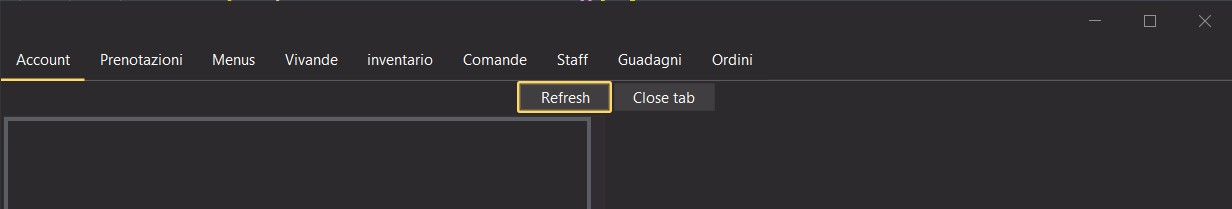
\includegraphics[width=\linewidth]{img/guide/tabs.jpg}
    \caption{Le pagine dell'interfaccia grafica.}
\end{figure}
La maggior parte delle pagine sono divise a metà, a sinistra si trova la lista degli elementi che concerne la pagina mentre a destra un form che si può usare per modificare o aggiungere elementi. Inoltre ogni casella di elementi ha dei tasti per operare sul singolo elemento.
\begin{figure}[H]
    \centering
    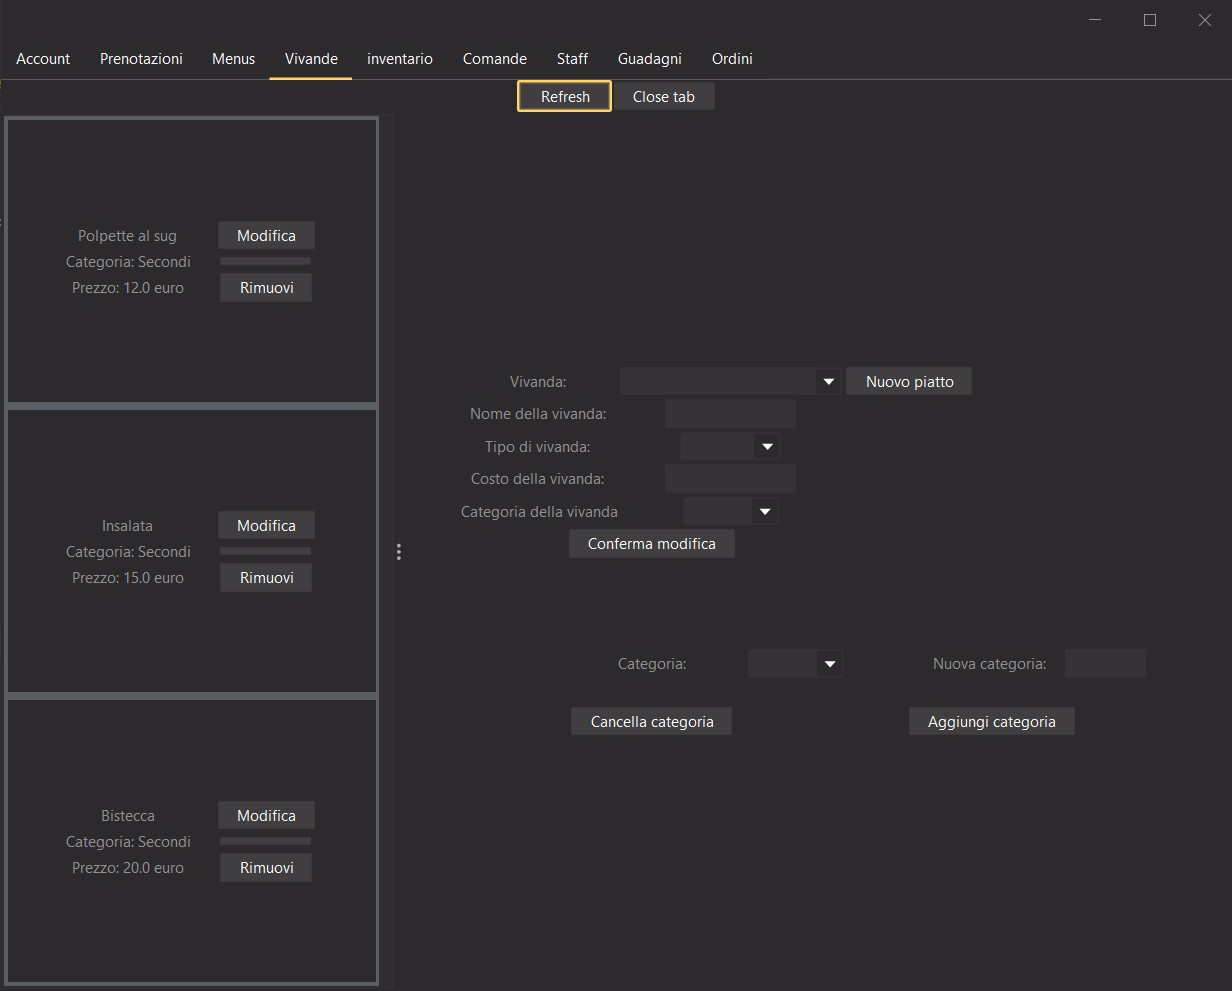
\includegraphics[width=\linewidth]{img/guide/foodtab.jpg}
    \caption{La pagina riguardante le vivande.}
    \label{foodtab}
\end{figure}
%
Vediamo in figura \ref{foodtab} che sulla sinistra i tasti "Modifica" e "Rimuovi" possono essere usati per rimuovere il singolo piatto o modificarlo. Alla pressione del tasto "Modifica" il form a fianco verrà riempito con le informazioni della vivanda e l'utente potrò modificarle.
\\
Inoltre è possibile anche aggiungere una nuova categoria di piatti o rimuovere quelle presenti.
\section{Log in e utenti}
Ogni utente ha un ruolo specifico deciso al momento della creazione dell'account. Il ruolo permette di fare uso di certi componenti del sistema come i menù, l'inventario... etc. Al momento del login l'utente vedrà aprire le schermate di suo interesse.
\\
Gli utenti che sono amministratori possono operare su tutte le finestre previste.
\begin{figure}[H]
    \centering
    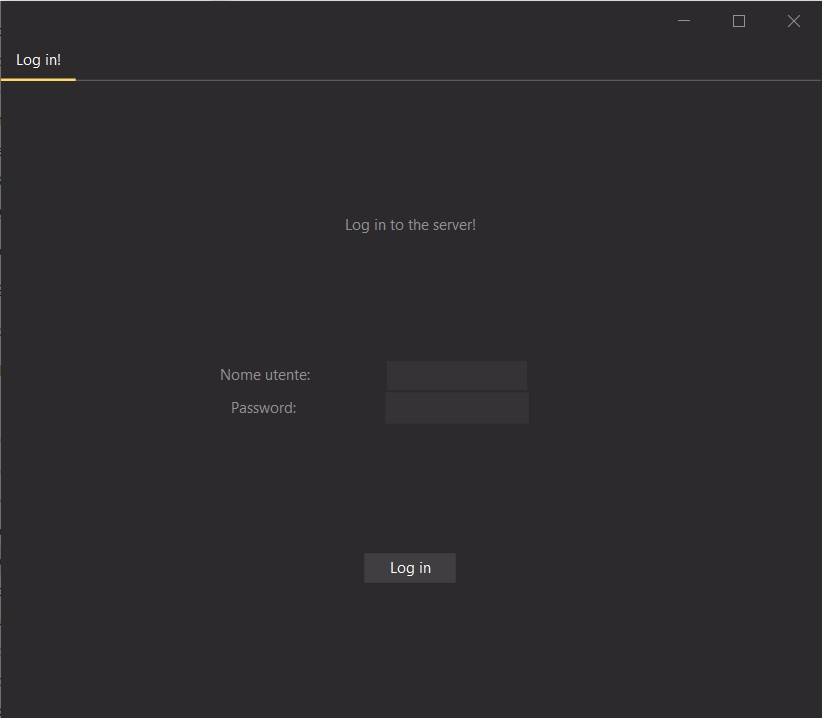
\includegraphics[width=0.7\linewidth]{img/guide/login.jpg}
    \caption{La schermata di login.}
\end{figure}
\end{document}
